\documentclass{article}
\usepackage[UTF8]{ctex}
\usepackage{float,indentfirst,verbatim,fancyhdr,graphicx,listings,longtable,amsmath, amsfonts,amssymb}

\textheight 23.5cm \textwidth 15.8cm
\topmargin -1.5cm \oddsidemargin 0.3cm \evensidemargin -0.3cm

\title{数值代数实验报告4}
\author{马天开}

\begin{document}
\maketitle

\section{问题描述}
\subsection{考虑两点边值问题}
\[
    \left\{
        \begin{aligned}
        & \epsilon \frac{d^2y}{dx^2}+\frac{dy}{dx}=a , 0 < a < 1, \\
        & y(0) = 0, y(1) = 1
        \end{aligned}
    \right.
\]

容易知道它的精确解为
\[
    y=\frac{1-a}{1-e^{-\frac{1}{\epsilon}}}1-e^{-\frac{x}{\epsilon}}+ax
    \]

为了把微分方程离散化,把 [0, 1] 区间 n 等分,令 $h = \frac{1}{n}, x_i = ih, i = 1,\cdots, n-1$, 得到差分方程
\[
    \epsilon \frac{y_{i-1}-2y_i+y_{i+1}}{h^2}+\frac{y_{i+1}-y_i}{h}=a
\]

简化为
\[
    (\epsilon + h)y_{i+1}-(2\epsilon + h)y_i + \epsilon y_{i-1} = ah^2
\]

离散化后得到线性方程组 Ay = b, 其中
\[
    A=\begin{bmatrix}
    \;-(2\epsilon + h) & (\epsilon + h) & 0 & 0 & \cdots & 0 \;\\
    \;\epsilon & -(2\epsilon + h) & (\epsilon + h) & 0 & \cdots & 0 \;\\
    \;0 & \epsilon & -(2\epsilon + h) & (\epsilon + h) & \cdots & 0 \;\\
    \;\vdots & & \ddots & \ddots & \ddots \;\\
    \;0 & \cdots & 0 & \epsilon & -(2\epsilon + h) & (\epsilon + h)\;\\
    \;0 & 0 & \cdots & 0 & \epsilon & -(2\epsilon + h)\;
    \end{bmatrix}
\]

\textbf{注意A为n-1阶矩阵,将线性方程组与差分方程进行对比得出正确的 b 向量(尤其注意第一行和最后一行)。}

对 $\epsilon = 1, a = 1/2, n = 100$, 分别用 Jacobi 迭代法,G-S 迭代法和 SOR 迭代法求线性方程
组的解,要求 4 位有效数字,然后比较迭代次数,运行时间与精确解的误差。迭代法终止条件为$||x^{(k+1)}-x^{(k)}|| < 10^{-6}$。

对 $\epsilon = 0.1, 0.01, 0.0001$, 考虑同样的问题。要求输出计算结果,收敛所需要的迭代次数和运行时间。


\subsection{考虑偏微分方程}
\[
    -\Delta u+g(x,y)u=f(x,y) \quad(x,y)\in [0,1]×[0,1]
\]


在[0,1]×[0,1]边界上 u = 1. 沿 x 方向和 y 方向均匀剖分 N 等份,令 h = 1/N, 并设应用中心差分离散化后得到差分方程的代数方程组为
$$-u_{i-1,j}-u_{i,j-1}+(4 + h^2g(ih, jh))u_{i,j}-u_{i+1,j}-u_{i,j+1} = h^2f(ih, jh)$$

取 $g(x, y) = \exp(xy)$, $f(x, y) = x+y$, 分别用Jacobi 迭代法,G-S 迭代法和 SOR 迭代法求解上述代数方程组,
要求输出解的最小分量,并比较 N = 20, 40, 60 时收敛所需要的迭代次数和运行时间,
迭代终止条件为 $||u^{(k+1)}-u^{(k)}||_2 < 10^{-7}$。

\textbf{要求仿照下面写的 Jacobi 迭代格式的推导过程推导处 G-S 迭代和 SOR迭代的格式},
在用 SOR 迭代法求解的过程中,请对不同的 N 使用合适
的松弛因子 $\omega$, 并在程序输出中打印松弛因子的值。观察运行结果后选取合适的。
(代码中不需要体现选取过程,只需给出即可)。

\textbf{注意本题中的三个迭代法的算法需要重新写,不能用矩阵的通用算法!!!}

\section{算法说明}

1、Jacobi 迭代法

考虑其迭代格式 $Dx_{(k+1)} = (L + U)x_k + b$。 对第 i 行有
\[
    D_iix_i^{(k+1)} =\sum_{i,j}(L + U)_{ij}x_j^{(k)} + b_i
\]
将D, L, U 还原成代数方程组的 Jacobi 迭代式

\[
    D_{ii}x_{i}^{(k+1)}= L_{i1}x^{(k)}_1 + \cdots + L_{ii-1}x^{(k)}_{i-1} + U_{ii+1}x^{(k)}_{i+1} +\cdots U_{in}x^{(k)}_n b_i
\]

即只有与向量 b 的下标相同的位置替换成 $x^{k+1}$。

由此类比推广至矩阵(或者可以直接将矩阵拉直成向量),知代数方程组 (1) 的 Jacobi 迭代格式为
\[
    (4 + h^2g(ih, jh))u_{i,j}^{(k+1)}=u_{i-1,j}^{(k)}+u_{i,j-1}^{(k)}+u_{i+1,j}^{(k)}+u_{i,j+1}^{(k)}+h^2f(ih, jh)
\]

2、G-S 迭代法

\[
    (4 + h^2g(ih, jh))u_{i,j}^{(k+1)} = u_{i-1,j}^{(k+1)} + u_{i,j-1}^{(k+1)} + u_{i+1,j}^{(k)}+u_{i,j+1}^{(k)}+h^2f(ih, jh)
\]

3、 SOR 迭代法

\[
    u_{i,j}^{(k+1)} = \dfrac{\omega}{4 + h^2g(ih, jh)} (u_{i-1,j}^{(k+1)} + u_{i,j-1}^{(k+1)} + u_{i+1,j}^{(k)}+u_{i,j+1}^{(k)}+h^2f(ih, jh)) + (1-\omega) u_{i,j}^{(k)}
\]

\section{程序介绍}
并没有什么特别值得介绍的,也许。这次抢了点ddl有的地方可能乱一点,见谅。

\newpage
\section{运行结果}

\verbatiminput{data/report_4_output.txt}

\newpage
\section{结果分析}

第一问画了个图,虽然没什么用,但是还是放上来了。
\begin{figure}[h]
    \centering
    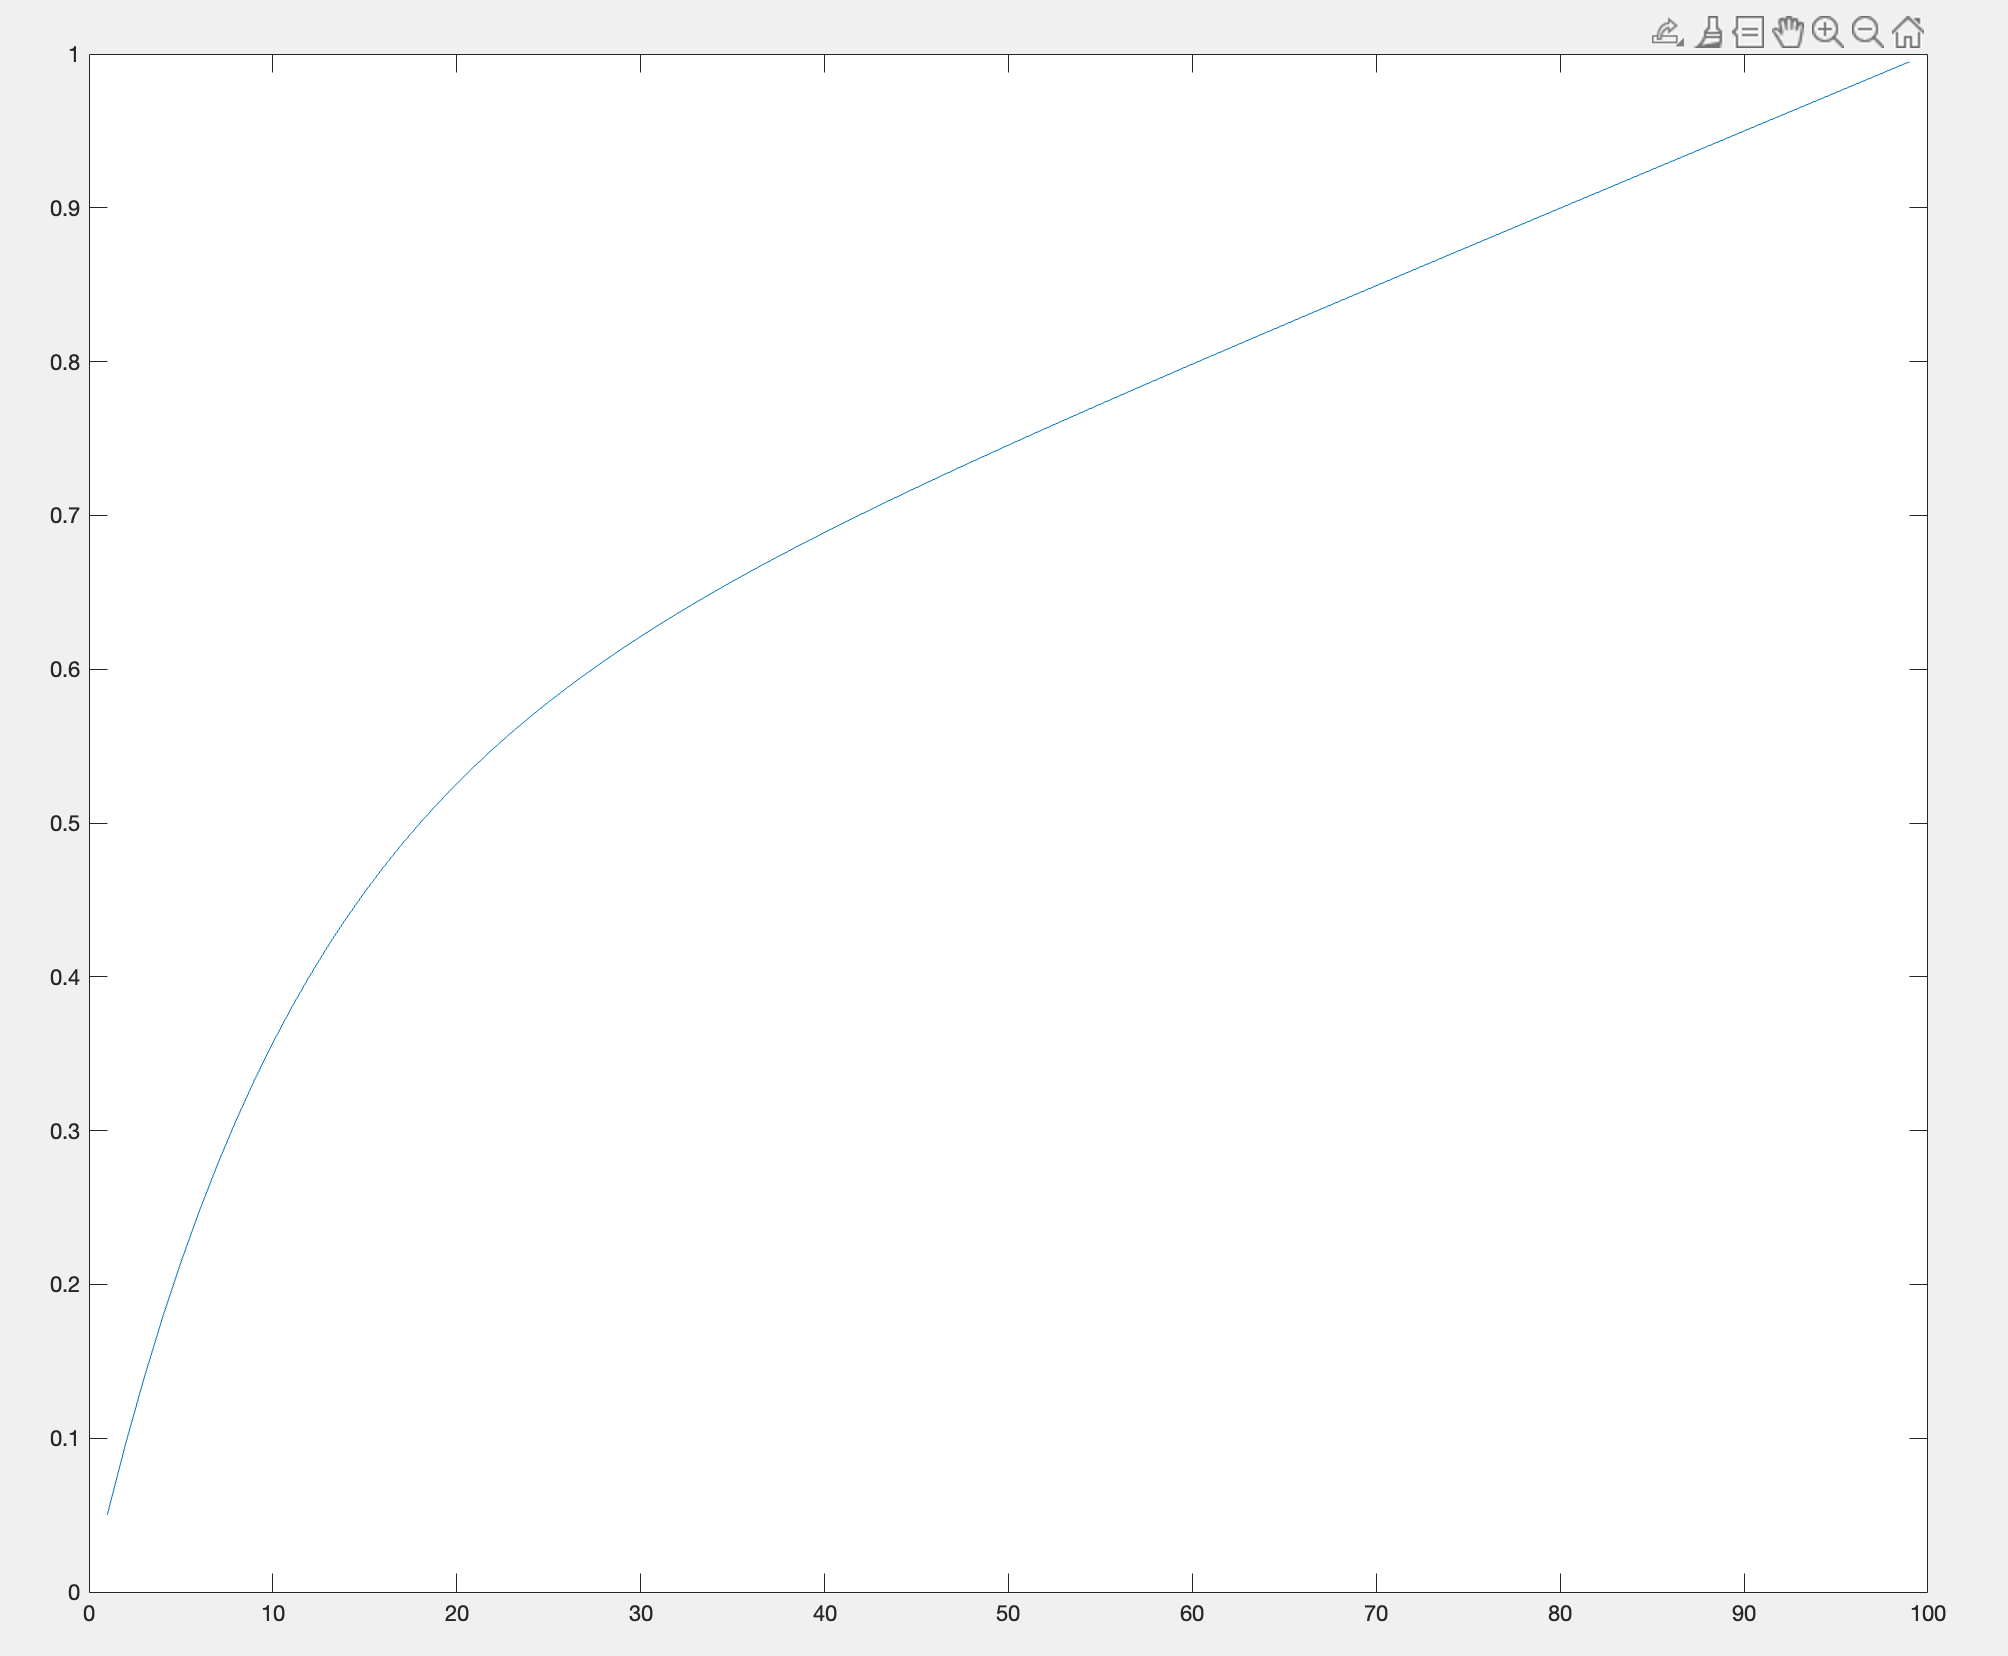
\includegraphics[width=0.5\textwidth]{img/4/matlab.png}
    \caption{计算数据}
\end{figure}

对比解析解绘制的图像:

\begin{figure}[h]
    \centering
    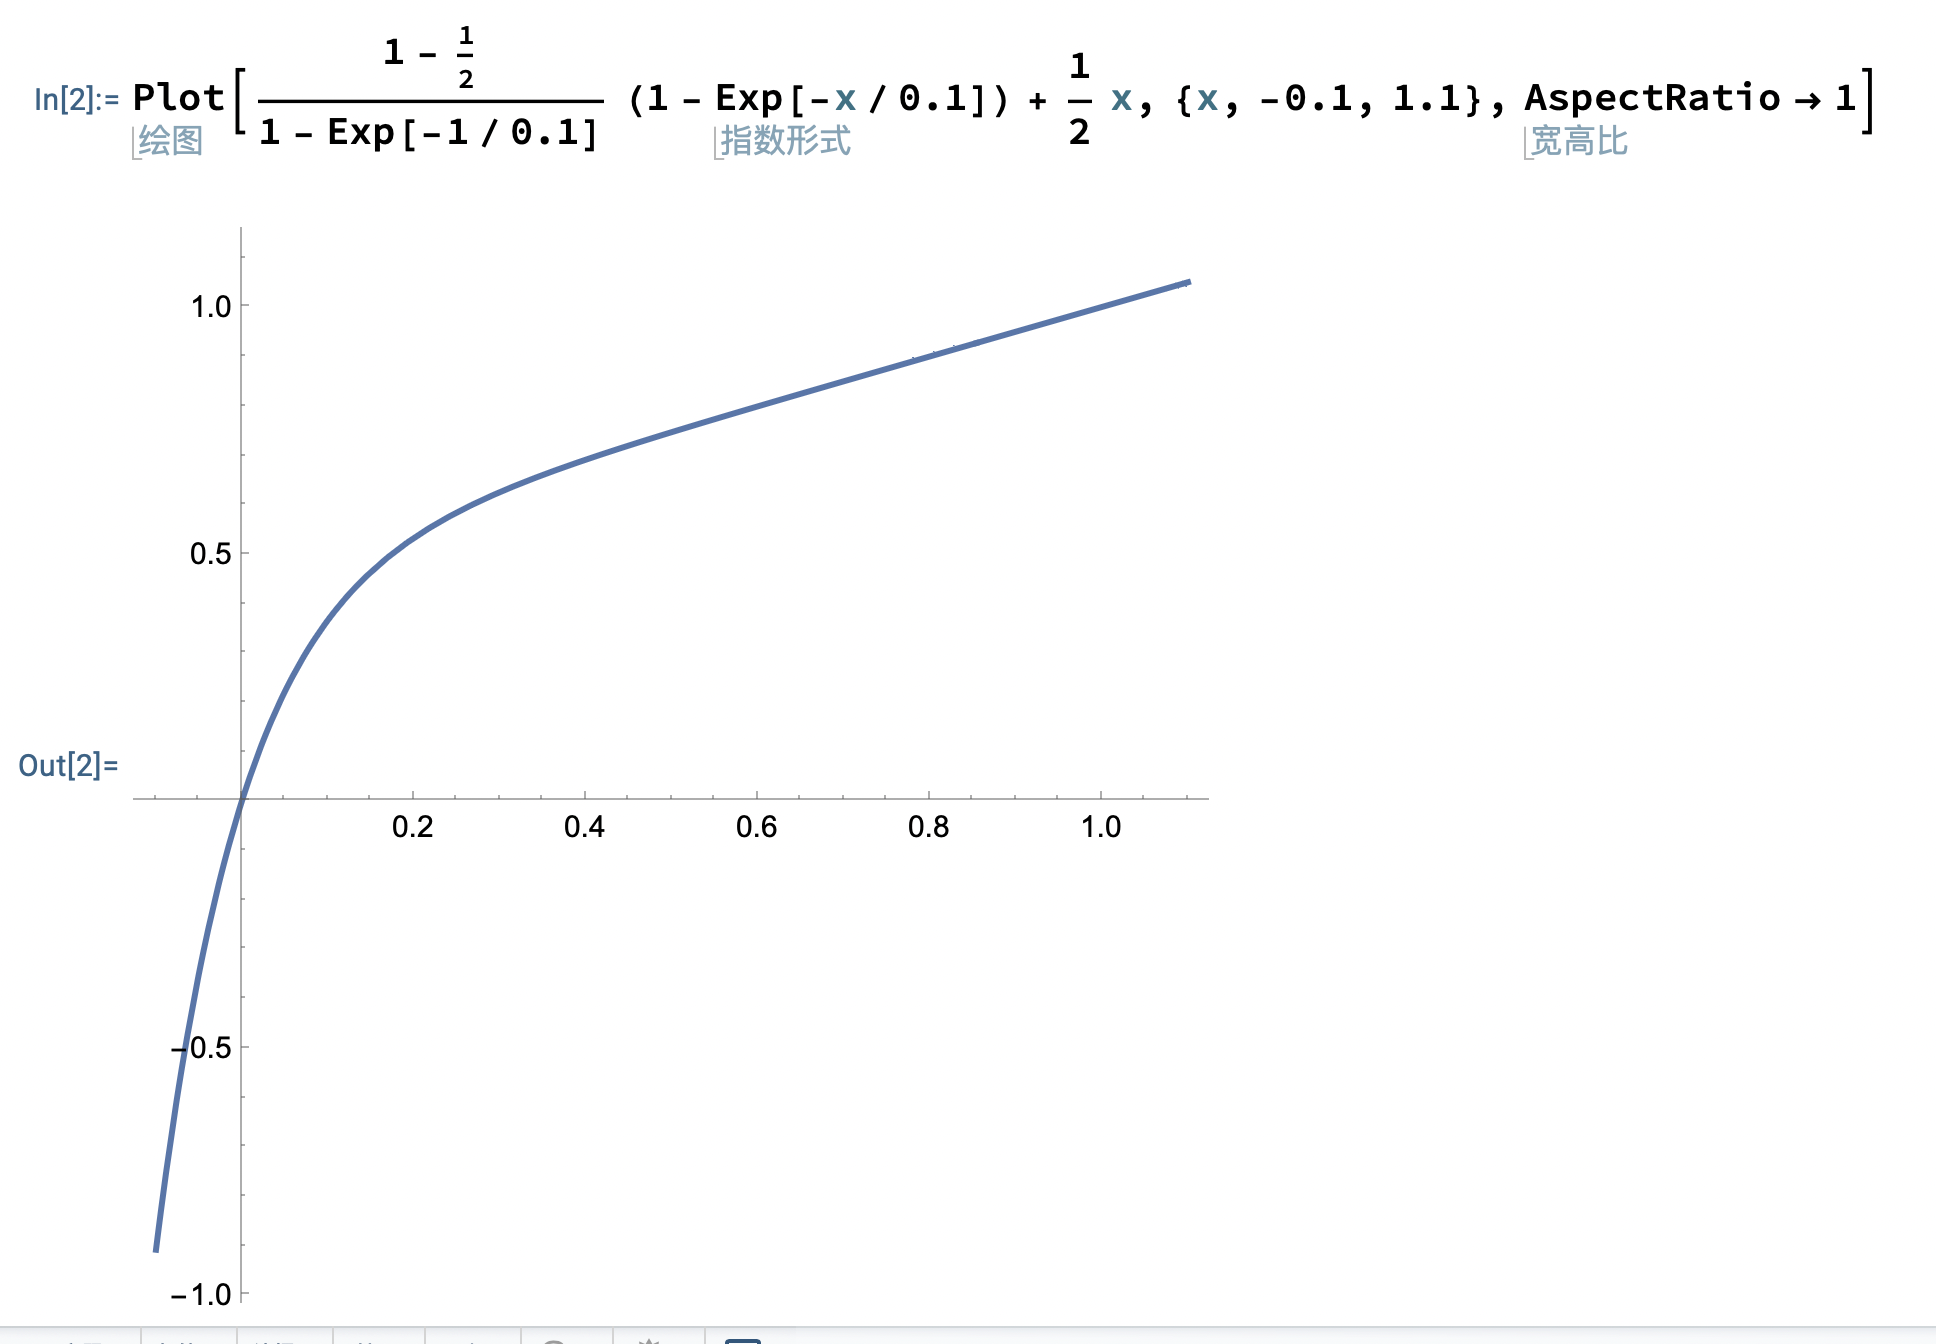
\includegraphics[width=0.8\textwidth]{img/4/mathematica.png}
    \caption{解析解}
\end{figure}

\end{document}